%%%%%%%%%%%%%%%%%%%%%%%%%%%%%%%%%%%%%%%%%%%%%%%%%%%%%%%%%%%%%%%%%%%%%%%%%%%%%%%%
% Chapter 1: Introducción
%%%%%%%%%%%%%%%%%%%%%%%%%%%%%%%%%%%%%%%%%%%%%%%%%%%%%%%%%%%%%%%%%%%%%%%%%%%%%%%%

% \textcolor{red}{texto}

%+++++++++++++++++++++++++++++++++++++++++++++++++++++++++++++++++++++++++++++++
En este capítulo se hablará sobre el estado y la situación en la que se
encuentra el tema a tratar en este Trabajo de Fin de Grado, y los objetivos
marcados.


%+++++++++++++++++++++++++++++++++++++++++++++++++++++++++++++++++++++++++++++++
\section{Antecedentes}
\label{1:sec:1}

Vivimos en una época emocionante para la ciencia y la ingeniería. Ya desde hace
200 años con el comienzo de la revolución industrial, se empezaron a cimentar
las primeras bases de la automatización de todas aquellas pequeñas tareas
repetitivas que eran un lastre para los tiempos de producción.

En el siglo XX la auténtica revolución ha llegado a través de la computación e
internet. La automatización en la computación ha sido, y es crucial, para el
desarrollo de nuevas líneas de trabajo como la inteligencia artificial.
Precisamente la inteligencia artificial y su implementación en la robótica ha
sido el último gran paso en los avances de la humanidad para optimizar,
sustituir o eliminar todo aquel trabajo tedioso, repetitivo o simplemente,
peligroso. Pero para ello se requiere del uso de todo tipo de sensores que
permitan simular el comportamiento de un ser humano.

La visión artificial es uno de los campos de investigación que más interés han
causado en las últimas décadas. Sin embargo, no ha sido hasta hace unos pocos
años cuando se ha empezado a conseguir los resultados esperados durante todo
este tiempo. El uso de cámaras permite obtener mucha y variada información
acerca del entorno de un robot: objetivos, obstáculos e incluso muchos datos que
aportan información directa de la situación que se visualiza.


%+++++++++++++++++++++++++++++++++++++++++++++++++++++++++++++++++++++++++++++++
\section{Estado del arte}
\label{1:sec:2}
% https://www.google.com/selfdrivingcar/
% https://en.wikipedia.org/wiki/Google_self-driving_car
Se ha demostrado que la mayoría de accidentes de tráfico tienen origen en el
factor humano, la visión artificial está muy presente en la actualidad en
sistemas guiados de vehículos autónomos, es decir, vehículos que son capaces de
conducir sin intervención humana, con el objetivo de minimizar estos sucesos.

\begin{wrapfigure}{l}{0.5\textwidth}
  \vspace{-20pt}
  \begin{center}
    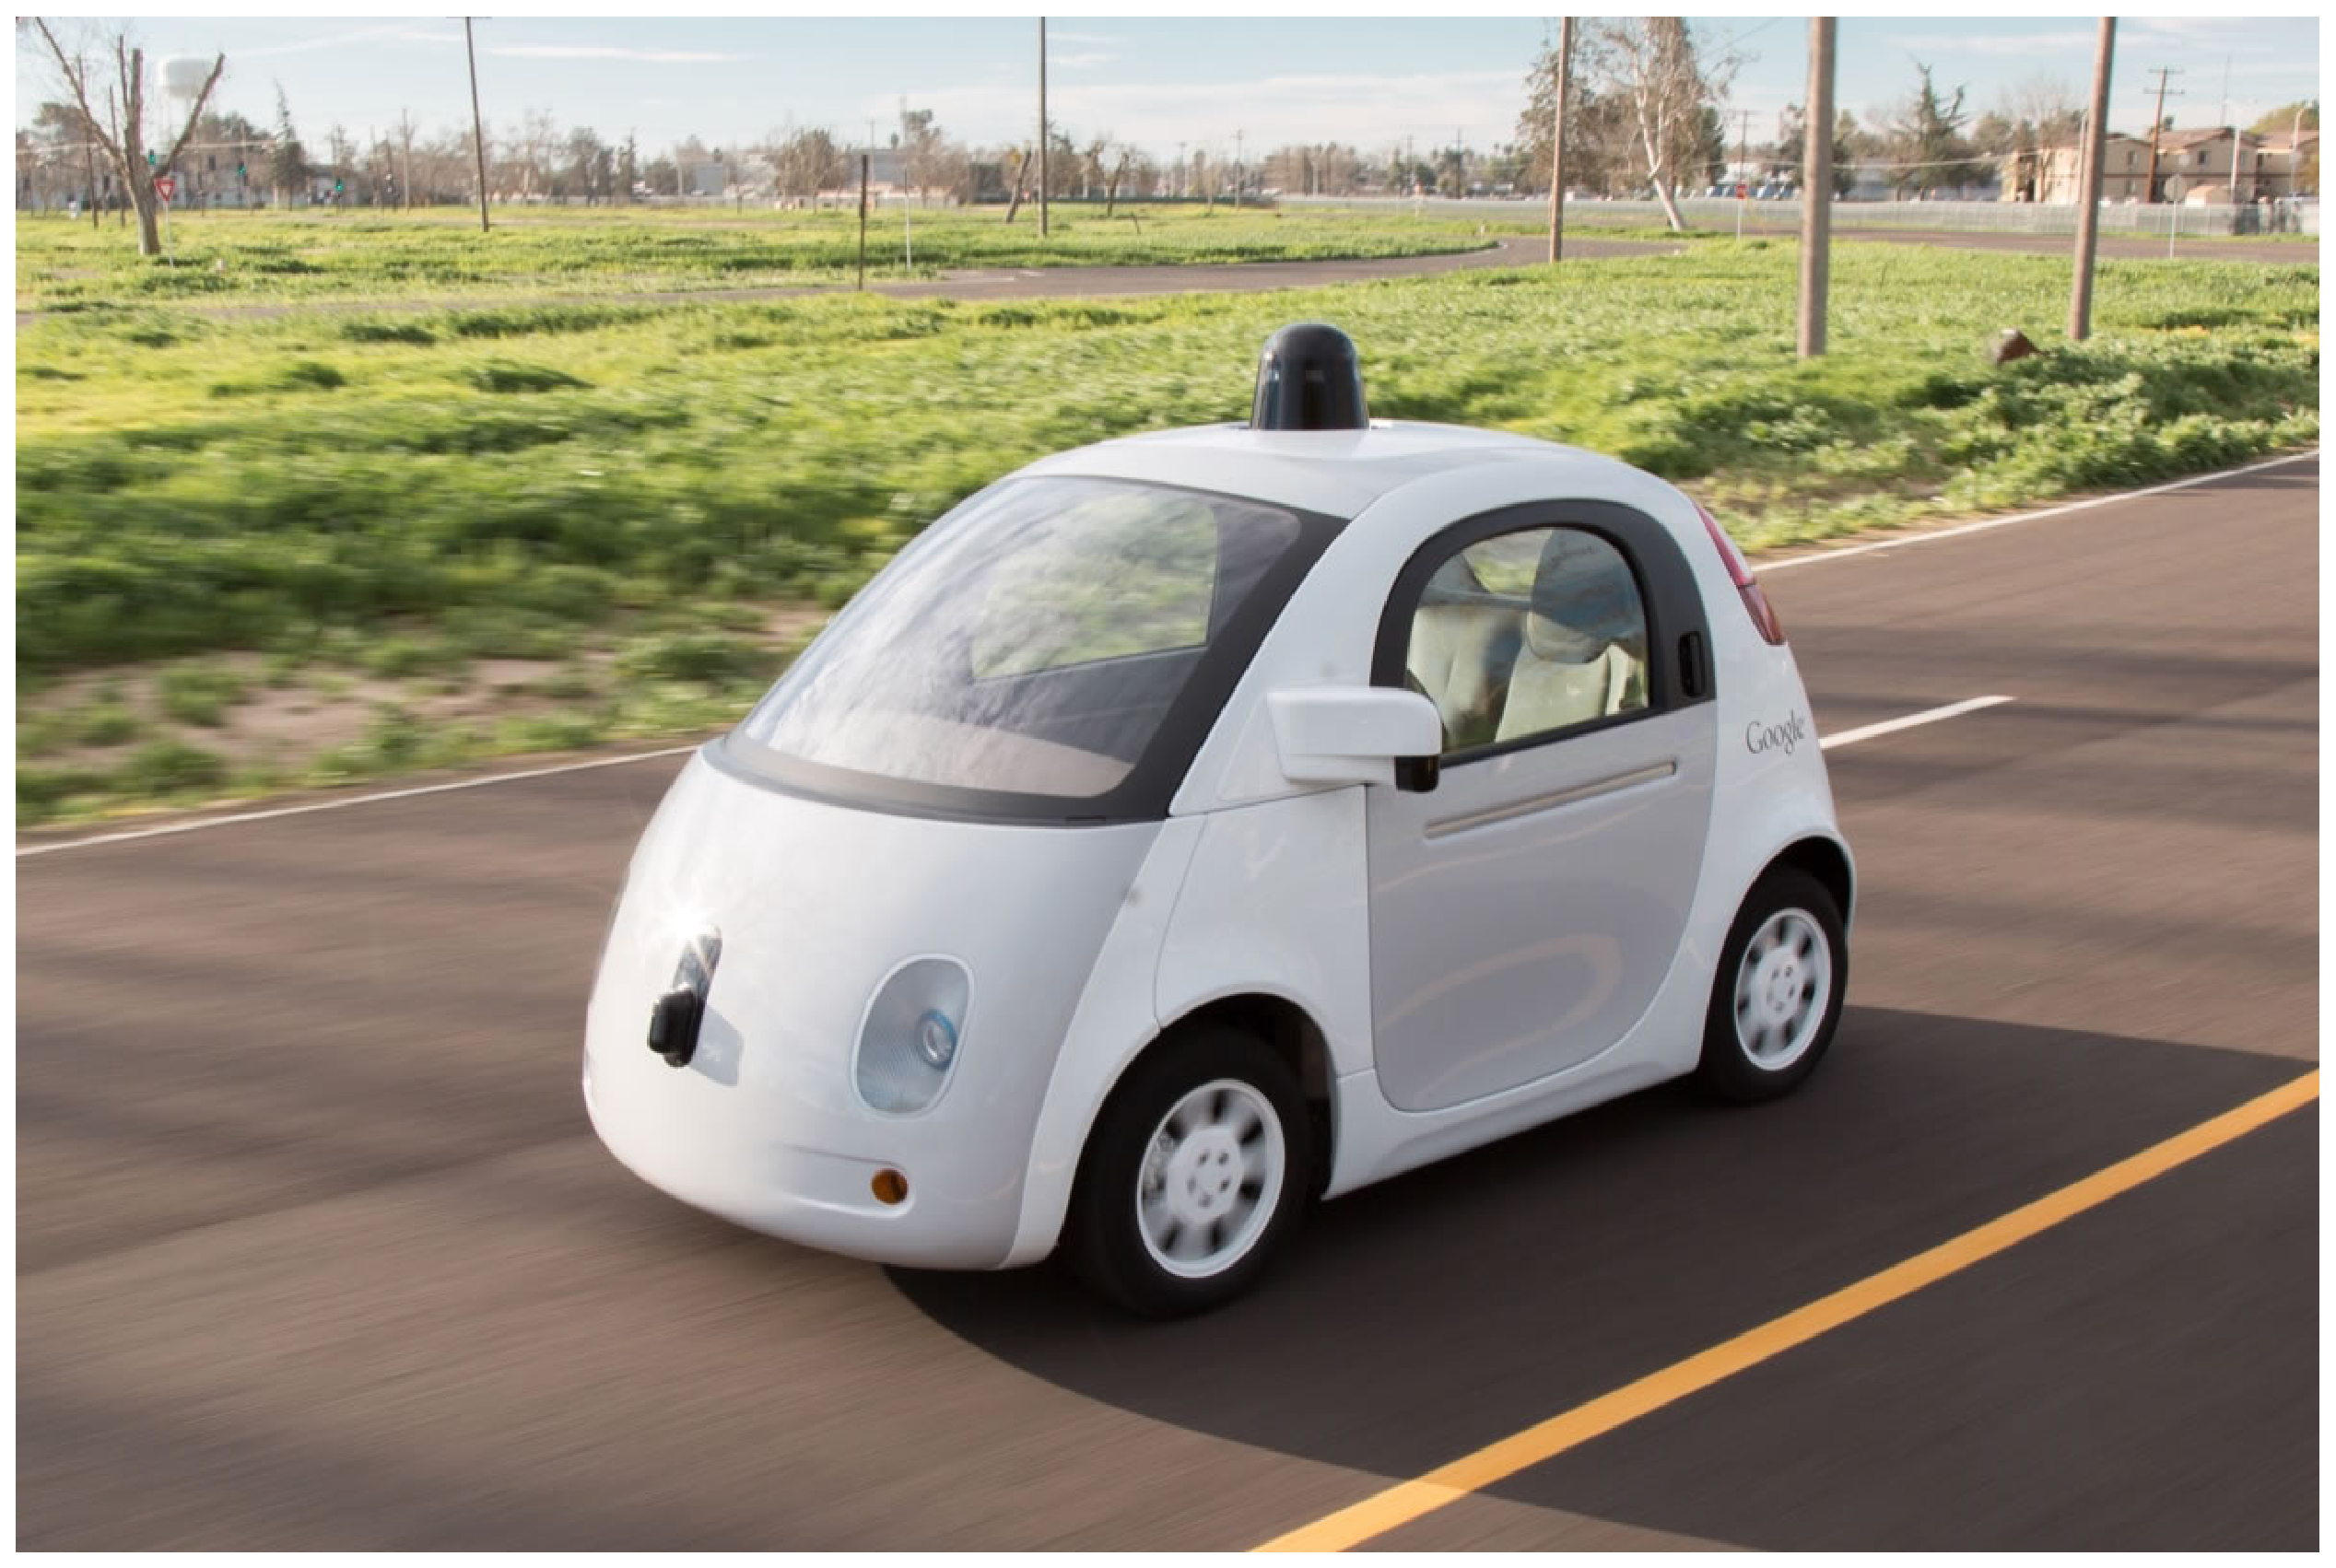
\includegraphics[width=0.48\textwidth]{images/cap1/GoogleSelf-DrivingCar.eps}
  \end{center}
  \vspace{-20pt}
  \caption{Google Self-Driving Car}
  \vspace{-10pt}
  \label{fig:GoogleSelf-DrivingCar}
\end{wrapfigure}

El ejemplo más conocido es el Google Self-Driving Car, un
vehículo totalmente autónomo que tras varios años de investigación, desde 2011
ya es legal su circulación en varios estados de Estados Unidos.

% http://verdino.webs.ull.es/
Por otra parte, la Universidad de La Laguna cuenta con el proyecto VERDINO,
desarrollado por el Grupo de Robótica (GRULL). Se trata de un vehículo similar
al de Google que hace uso de sistemas láser, sistemas de visión (tanto en el
espectro visible como infrarrojo) y sistemas de odometría óptica, entre otras
características. Todo ello para ser capaz de detectar el entorno que le rodea,
y poder realizar una toma de decisiones mediante el uso de diferentes algoritmos
para llegar hasta un destino, al mismo tiempo que preocupa por evitar los
obstáculos que aparecen en su camino.

\begin{wrapfigure}{r}{0.5\textwidth}
  \vspace{-20pt}
  \begin{center}
    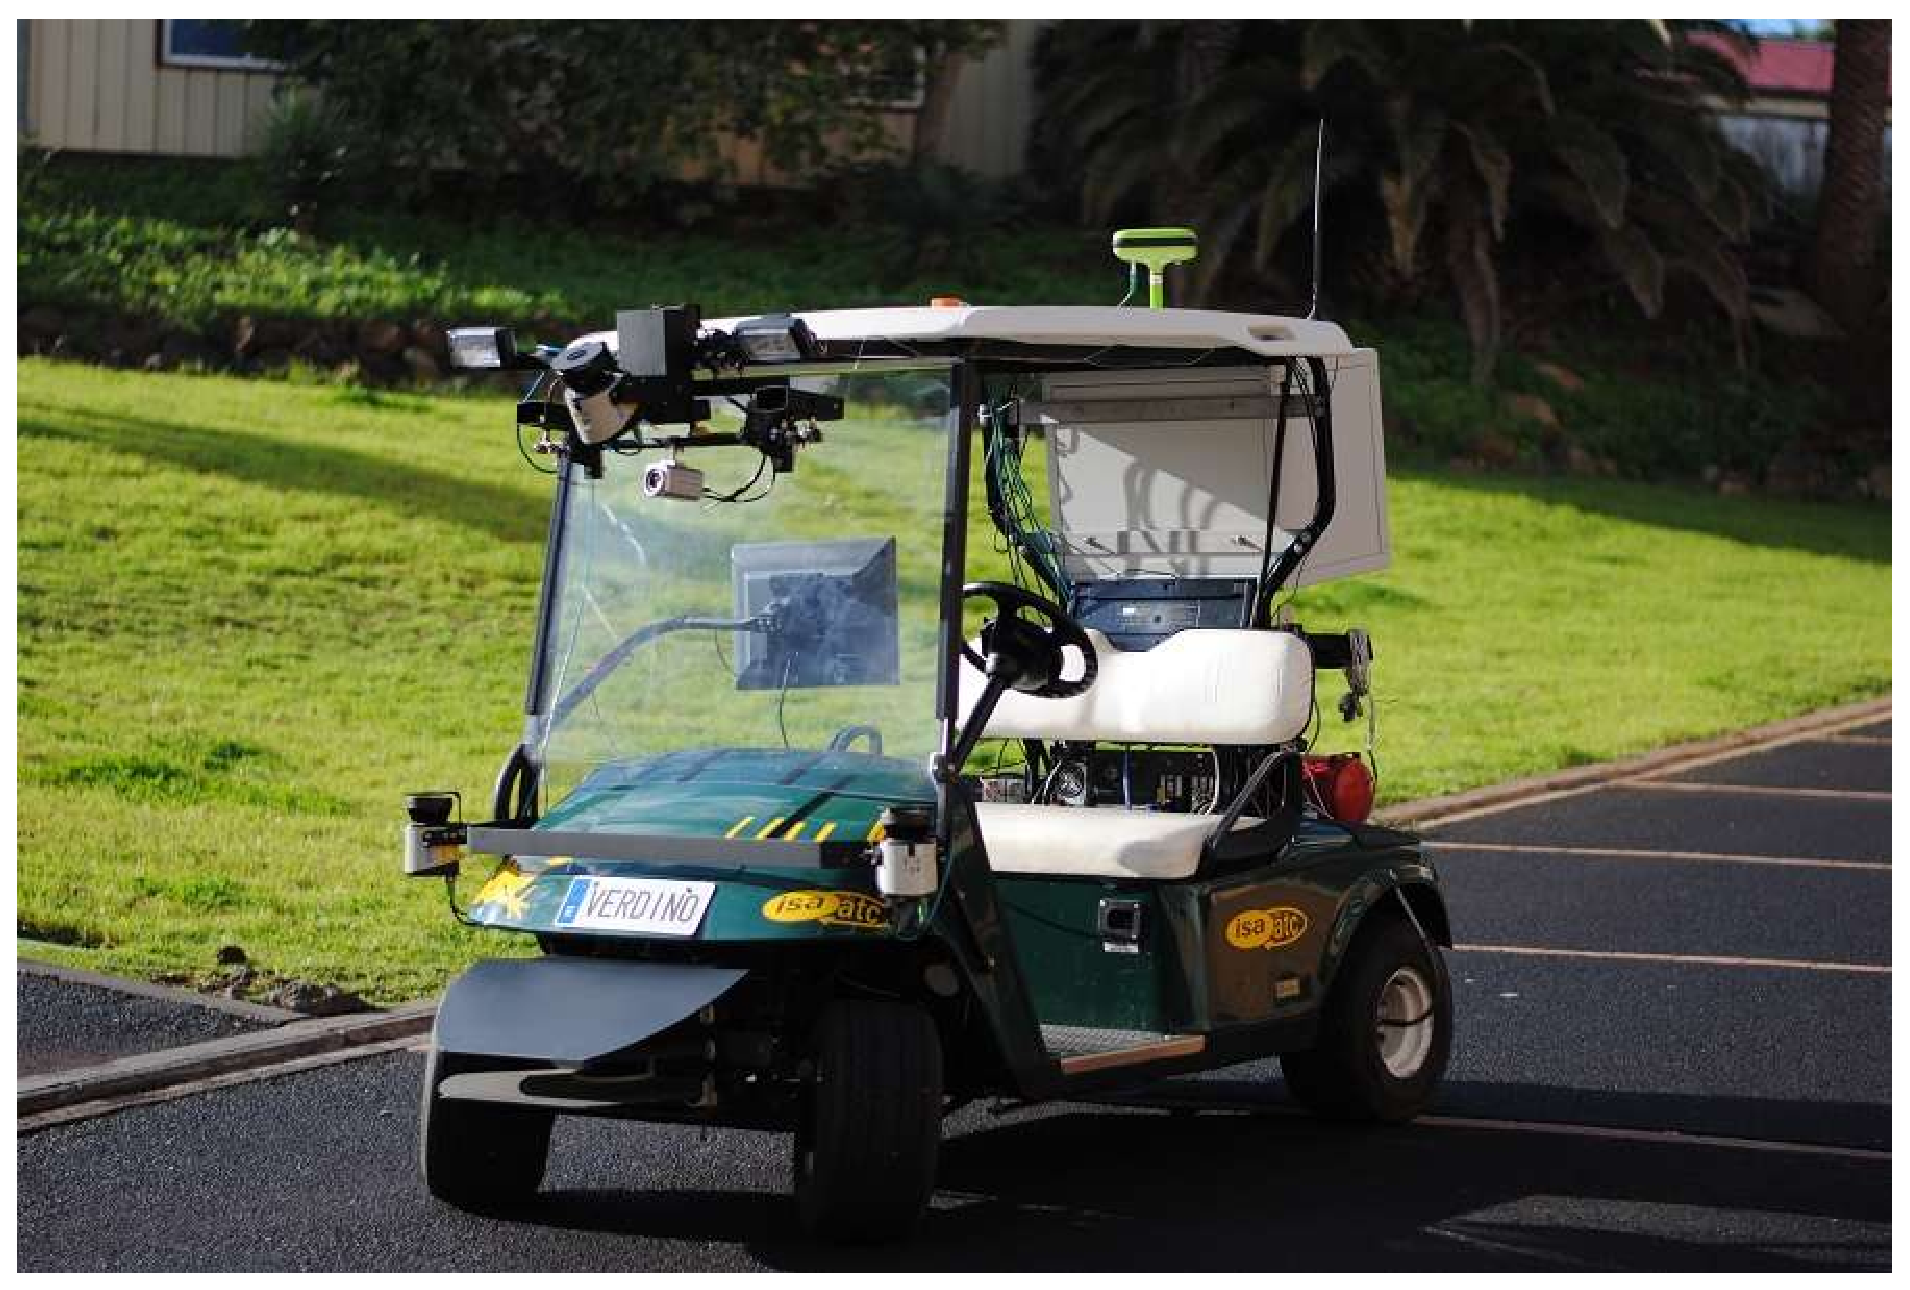
\includegraphics[width=0.48\textwidth]{images/cap1/Verdino.eps}
  \end{center}
  \vspace{-20pt}
  \caption{Proyecto VERDINO}
  \vspace{-10pt}
  \label{fig:ProyectoVERDINO}
\end{wrapfigure}

De momento es difícil predecir cuando se producirá la entrada masiva en el
mercado de este tipo de vehículos. Los dos proyectos mencionados anteriormente,
aunque fiables a pesar de seguir en desarrollo, hacen uso de tecnología poco
accesible para el público general debido a su elevado presupuesto.

Este problema abre las puertas a nuevas alternativas de investigación, a través
de tecnologías más limitadas que todavía no se han explotado en este campo, pero
que son igual de válidas. Es el caso de los sistemas de visión estereoscópica,
que con solamente dos cámaras se puede obtener rica información del entorno.


%+++++++++++++++++++++++++++++++++++++++++++++++++++++++++++++++++++++++++++++++
\section{Objetivo}
\label{1:sec:3}

El tema central de este proyecto es muy ambicioso, de este modo, es necesario
poder realizar una distinción entre el objetivo principal y los objetivos
específicos que lo rodean.

%--------------------------------------
\subsection{Objetivo general}

\textcolor{red}{¿Detección y esquiva o reconstrucción del mapa?}

El objetivo principal de este Trabajo de Fin de Grado es poder integrar el uso
de un sistema estereoscópico de dos cámaras en un robot, para la detección y
posteriormente esquiva de los obstáculos que se encuentren mediante la
construcción de un mapa tridimensional como referencia.

%--------------------------------------
\subsection{Objetivos específicos}

Los objetivos específicos que componen el proyecto son:
% \newline
\begin{itemize}
  \item Uso de una cámara comercial de entretenimiento en un proyecto de
  investigación.
  \item Reconstrucción de un mapa tridimensional a partir de las imágenes
  recogidas por las cámaras.
  \item Integración de cámaras estereoscópicas junto a otros sistemas de
  detección de obstáculos.
  \item Combinación de odometría mecánica y odometría láser.
\end{itemize}


%+++++++++++++++++++++++++++++++++++++++++++++++++++++++++++++++++++++++++++++++
% \label{1:sec:3}
% \begin{itemize}
%   \item Item 1
%   \item Item 2
%   \item Item 3
% \end{itemize}
% Bla, bla, bla

%+++++++++++++++++++++++++++++++++++++++++++++++++++++++++++++++++++++++++++++++
% \section{Sección Cuatro}
%   \label{1:sec:4}
%
% Bla, bla, bla

% \begin{figure}[!th]
%   \begin{center}
%     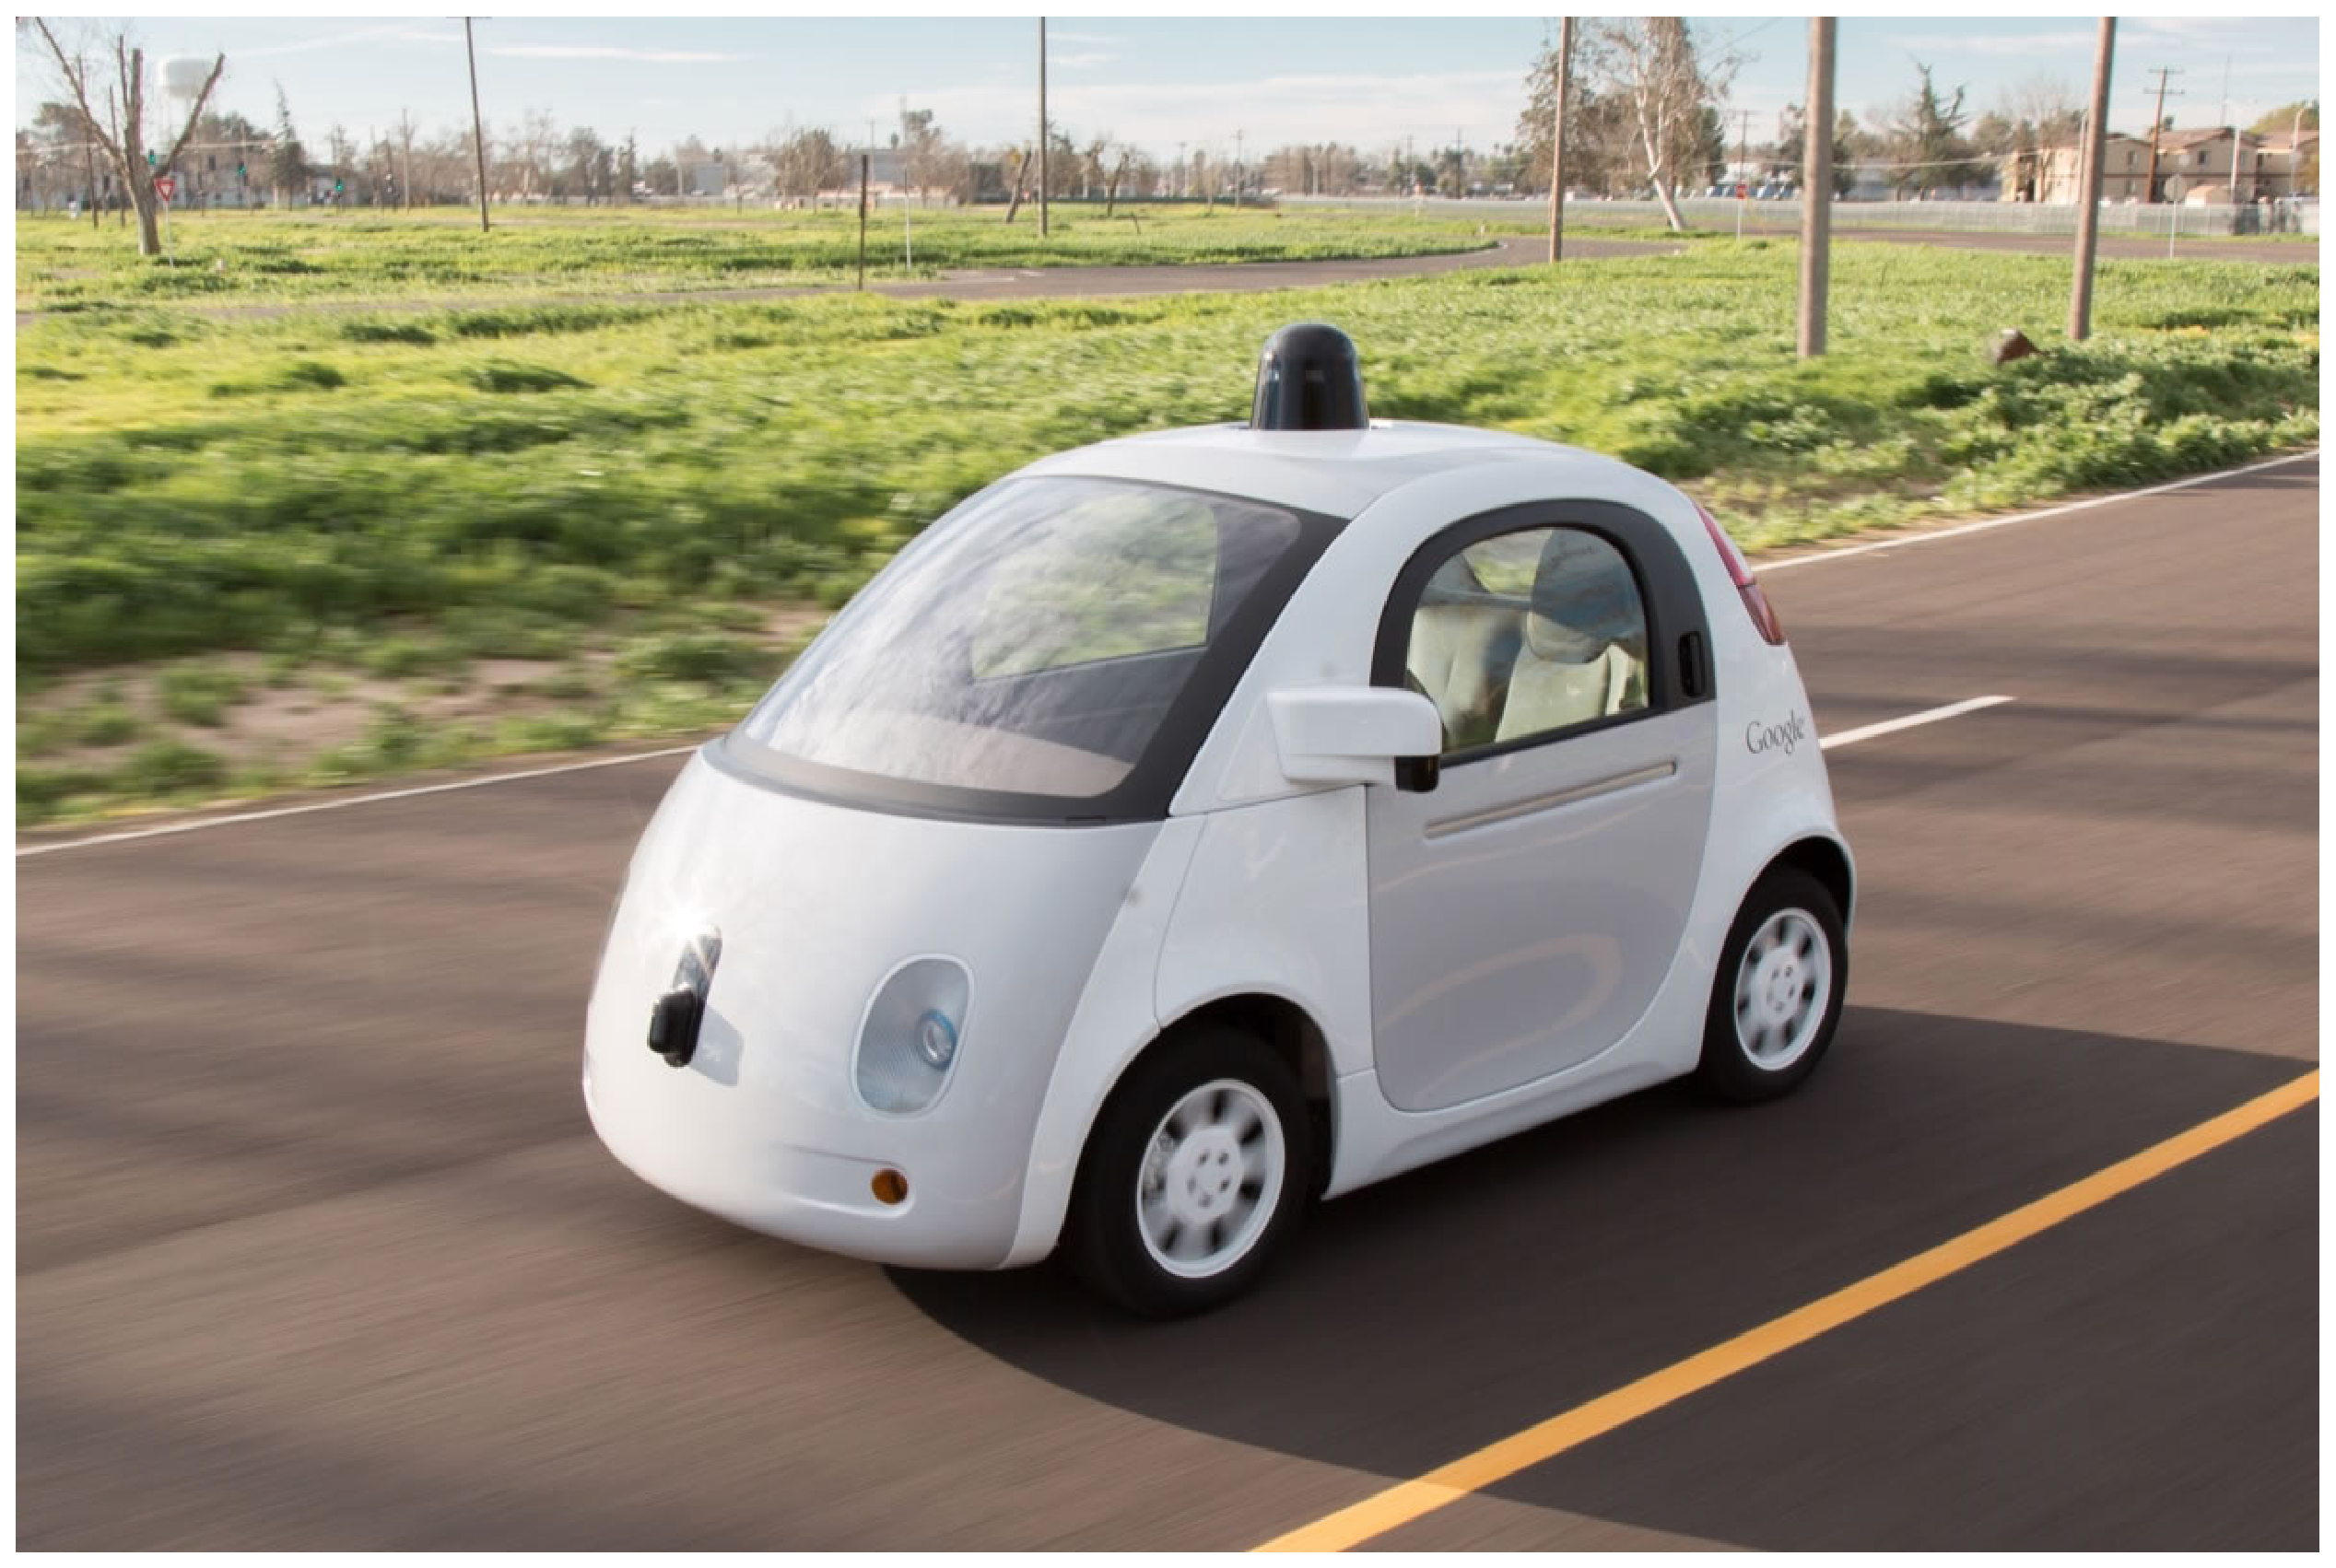
\includegraphics[width=0.5\textwidth]{images/cap1/GoogleSelf-DrivingCar.eps}
%     \caption{Google Self-Driving Car}
%     \label{fig:GoogleSelf-DrivingCar}
%   \end{center}
% \end{figure}

%+++++++++++++++++++++++++++++++++++++++++++++++++++++++++++++++++++++++++++++++
%+++++++++++++++++++++++++++++++++++++++++++++++++++++++++++++++++++++++++++++++
